\chapter{Algorithm Design} \label{chap3}
\subsubsection{Research of a Taxi Driver in the queue:}
This algorithm describes how the system manages the research of a taxi drivers. It will use the \textit{Dequeue} operation in order to extract the first taxi driver and the \textit{Call} function in order to propose him a ride. If the first taxi driver accepts the request, this will be assigned to him, otherwise he will be enqueued again using the \textit{Enqueue} operation and the system will use the new first element of the queue to detect the new taxi driver who will receive the request, and so on until a taxi driver accepts the request.

\begin{algorithm}[H]
\caption{Research of a Taxi Driver}
\begin{algorithmic}[1]
\Procedure{SearchTaxiDriver}{$Q$}
\If{$(Q.head == Q.tail)$}\Comment{Queue is empty}
	\Else
	\For{$i:= 0$ \textbf{to} $Q.lenght$}\Comment{The system knows the length of the Queue, so it makes exactly \textit{Q.length} controls}
		\State $x \gets Dequeue(Q)$\Comment{Classical operation for managing the extraction of an element from the Queue}
		\State $acceptance \gets Call(x)$\Comment{Function that represent the call that the system makes to the driver in order to propose a ride. It \textbf{returns true} if the taxi driver accepts the call and is willing to make the ride, otherwise \textbf{returns false} if the taxi driver declines the call}
		\If{$(acceptance == true)$}
			\State $\textbf{return} \: x$
		\Else
			\State $Enqueue(Q, x)$\Comment{Classical operation for managing the insertion of an element from the Queue}
		\EndIf
	\EndFor
\EndIf
\EndProcedure
\end{algorithmic}
\end{algorithm}

\subsubsection{Shared Ride Management:}
This is the algorithm that is responsible to manage the Shared Rides. Here there are some general information about the algorithm: \\
There is one sharing list per every taxi area ordered by the starting time of the ride. Match between elements of the list is done under a time window of 10 minutes after the selected starting time (for reservation) and after the moment of the call (for request).When is time to start assigning a driver to the request/reservation and start the ride, the system deletes the corresponding element from the list (is always the head of the list because of the ordering). There is also a buffer (Figure \ref{fig:buff}) to make sequential the adding of new requests/reservations to the list and avoid conflicts.\\
The flowchart diagram in Figure \ref{fig:genalg} represent the generic algorithm which describes how the system manage the functionality of "Ride Sharing".

\begin{figure}[htbp]
\centering
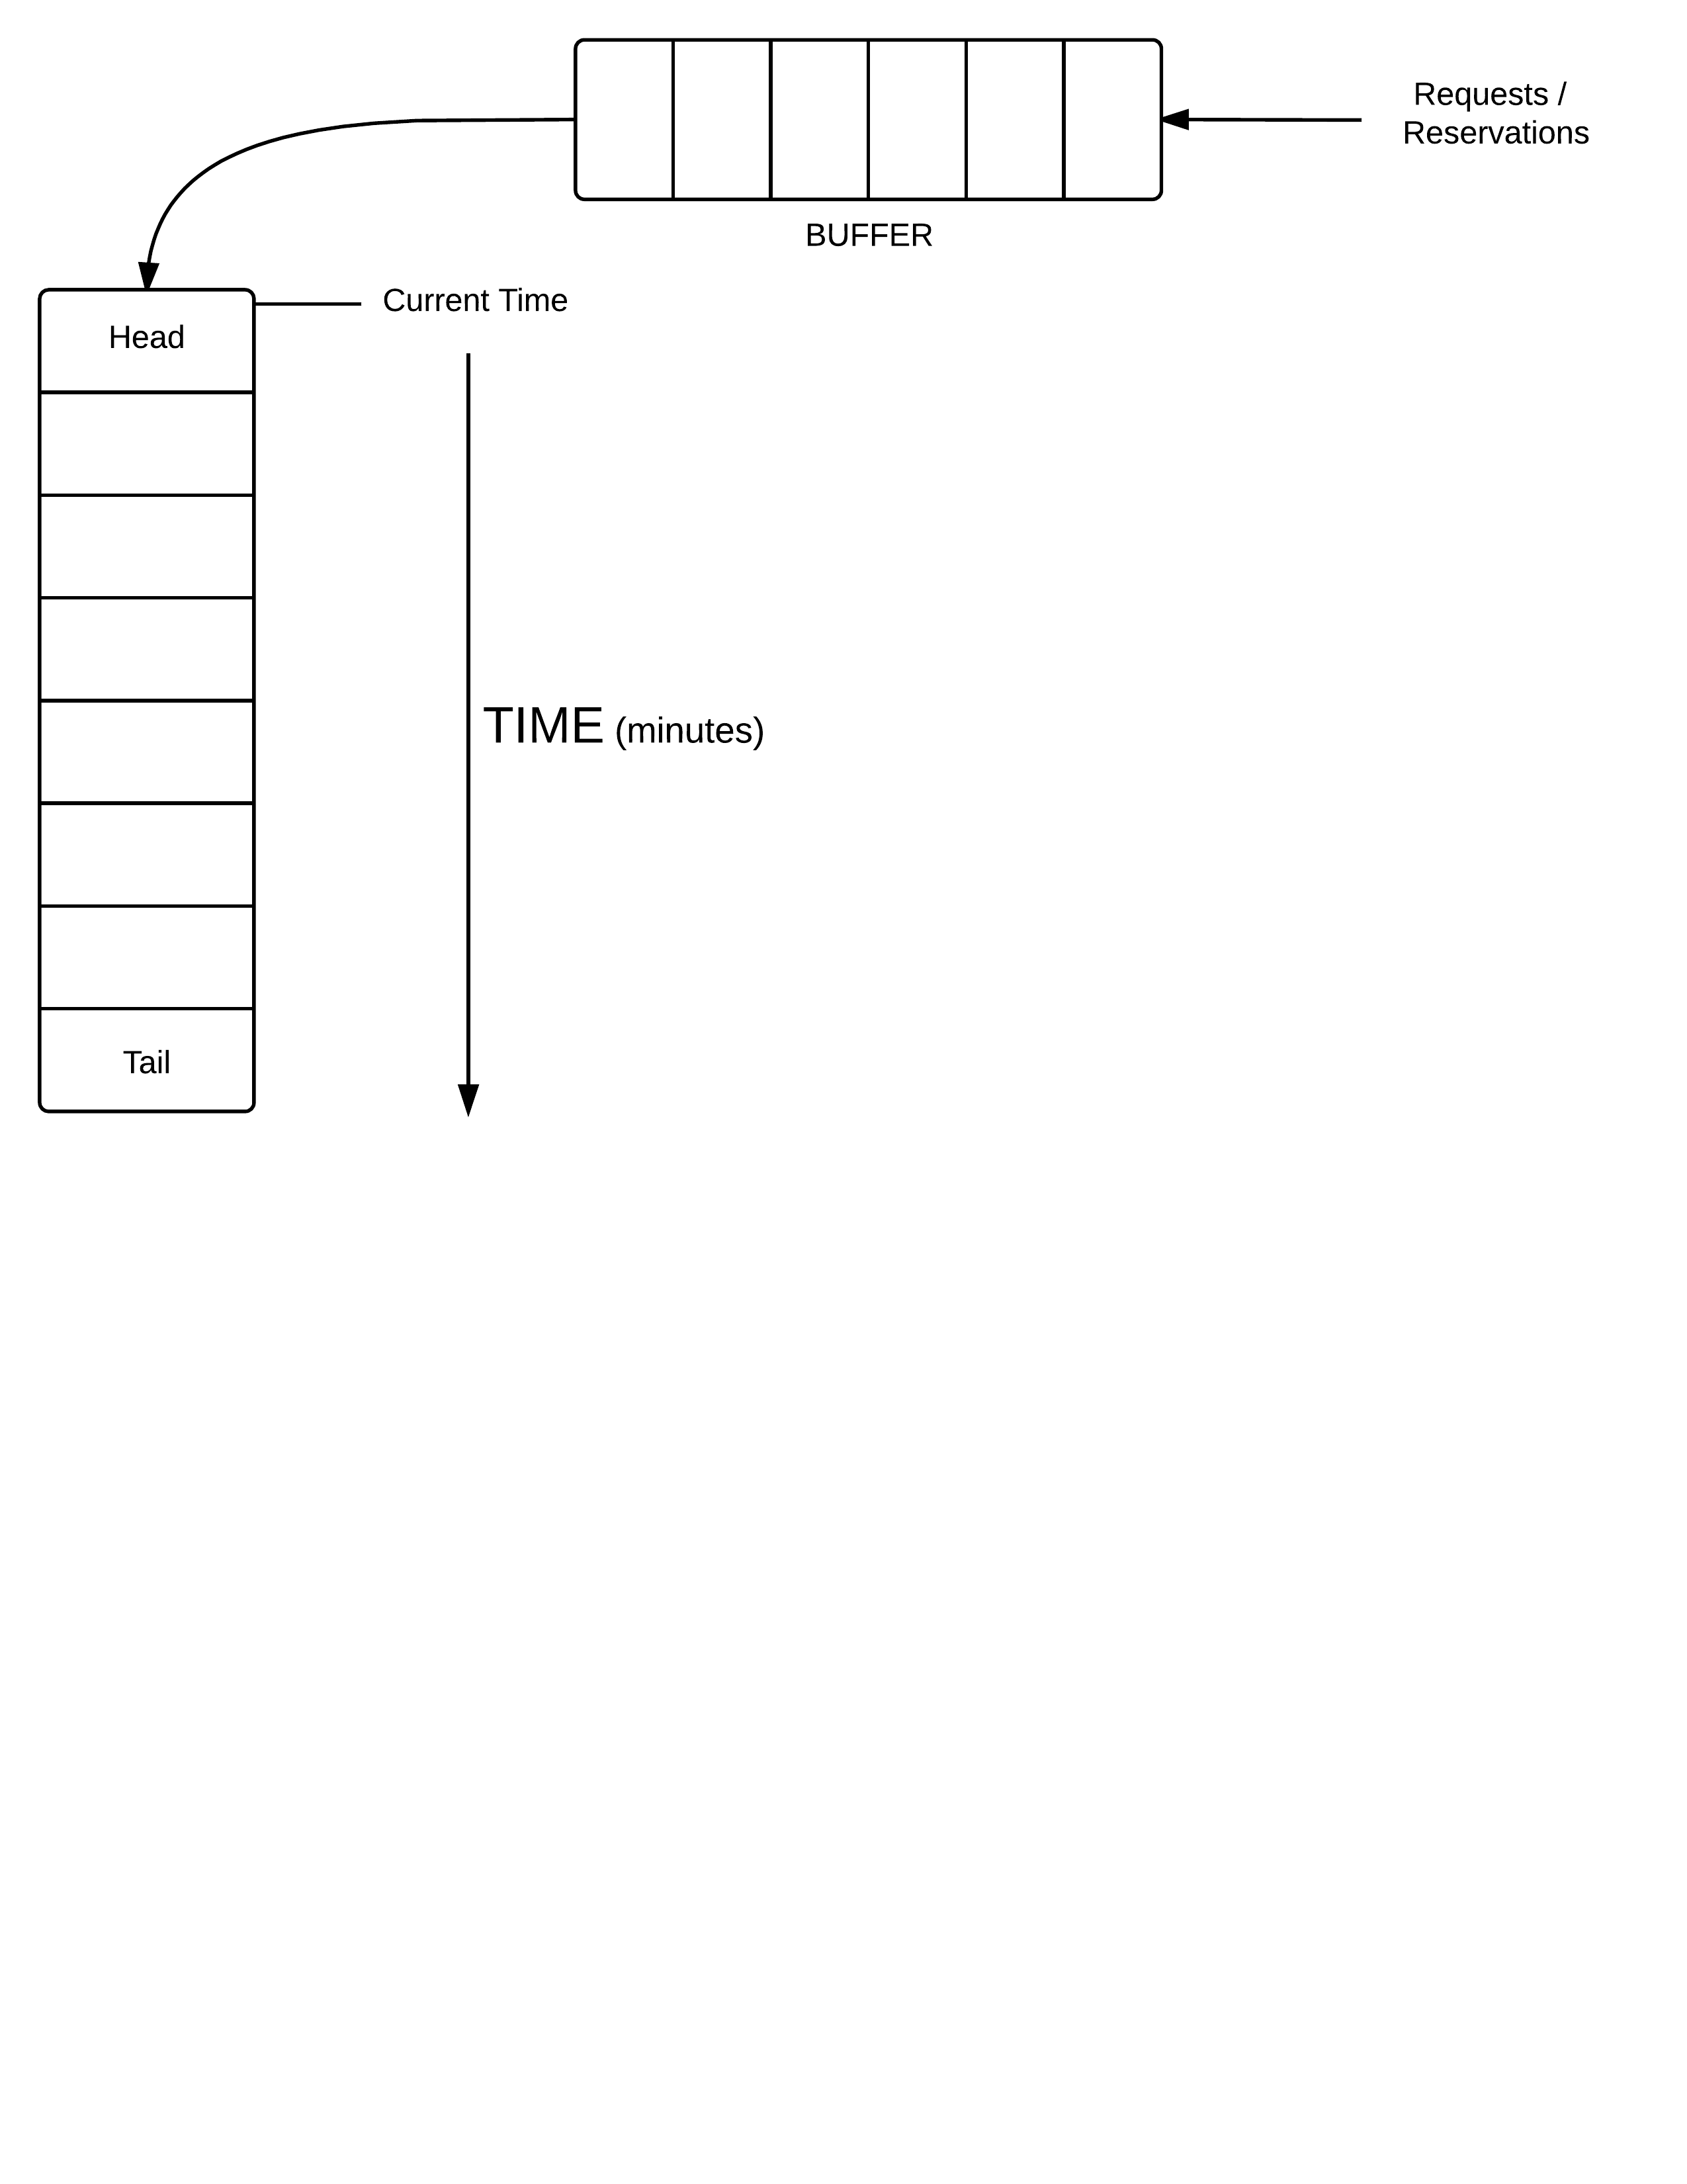
\includegraphics[width=\textwidth]{cpt/img/BufferQueue}
\caption{Representation of interaction between Queue and Buffer}
\label{fig:buff}
\end{figure}
\clearpage

\begin{figure}[htbp]
\centering
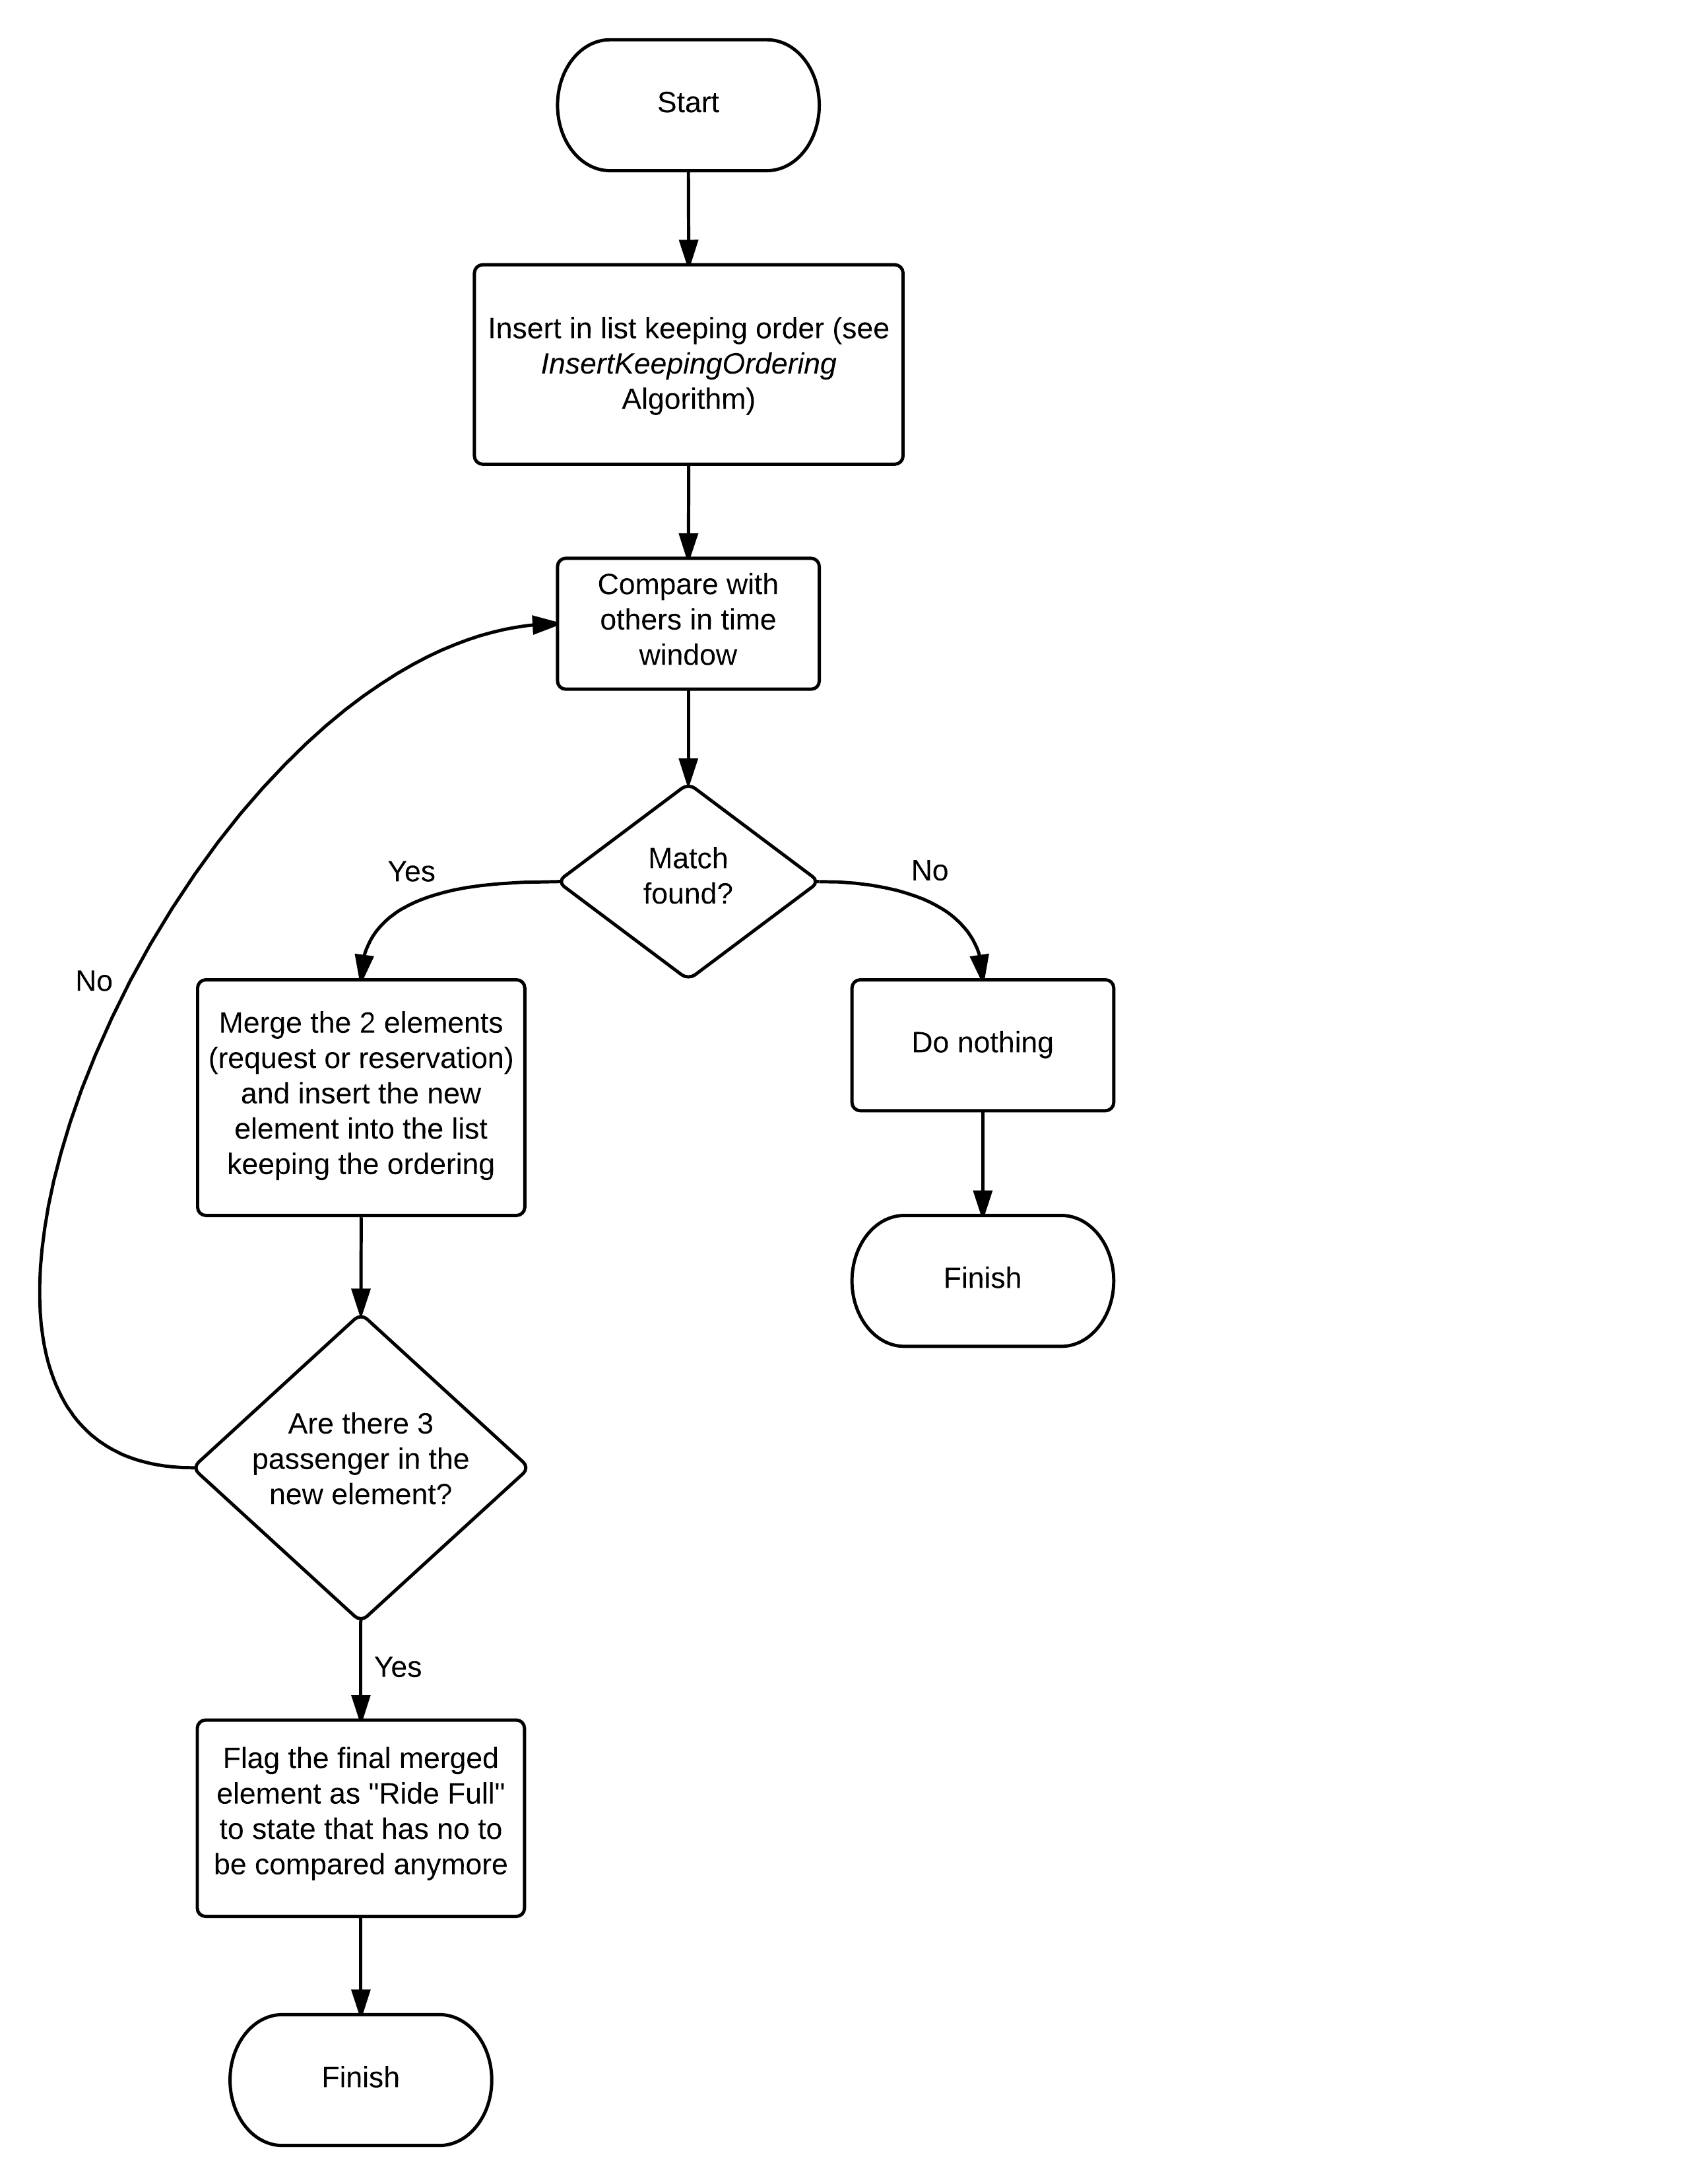
\includegraphics[width=\textwidth]{cpt/img/GenericAlgorithm}
\caption{Representation of the Shared Ride Management Algorithm}
\label{fig:genalg}
\end{figure}
\clearpage

The following algorithms describe in details the behavior of the list and how the Shared Ride Management Algorithm works:

\begin{algorithm}[H]
\caption{Check for Compatibility}
\begin{algorithmic}[1]
\Procedure{CheckForCompatibility}{$x, List$}
\For{$each \: element \: e \: \textbf{in} \: Sublist(x)$}\Comment{\textit{Sublist(x)} indicates the portion of the list starting from the successor of element \textit{x}}
	\If{$((e.startTime \leq x.startTime + 10)$ \textbf{\&\&} $(e.destinationArea == x.DestinationArea)$ \textbf{\&\&} $(e.flagAsFullRide == false))$}
		\State $\textit{MergeRides(x, e)}$
		\State ${\textbf{break()}}$
	\EndIf
\EndFor
\EndProcedure
\end{algorithmic}
\end{algorithm}

\begin{algorithm}[H]
\caption{Merge Rides}
\begin{algorithmic}[1]
\Procedure{MergeRides}{$x, y$}
\State \textit{Creates a new element z with the same originArea and destinationArea of x and y}
\If{$x.startTime < y.startTime$}
	\State $z.startTime \gets x.startTime$
	\Else
	\State $z.startTime \gets y.startTime$
\EndIf
\State \textit{All the other information about the request/reservation are copied from x and y into z}
\EndProcedure
\end{algorithmic}
\end{algorithm}

\begin{algorithm}[H]
\caption{Insert an element in List keeping the order}
\begin{algorithmic}[1]
\Procedure{InsertKeepingOrdering}{$x, List$}
\For{$each \: element \: e \: \textbf{in} \: List$}
	\If{$(e.startTime \geq x.startTime)$}
		\State $e.prev.next \gets x$\Comment{\textit{e.prev.next} indicates the attribute next of the element pointed by \textit{e.prev}}
		\State $x.prev. \gets e.prev$
		\State $x.next \gets e$
		\State $e.prev \gets x$
		\State ${\textbf{break()}}$
	\EndIf
\EndFor
\EndProcedure
\end{algorithmic}
\end{algorithm}